\chapter{Methods and Testing}

\begin{exercise}
Presume you are selling a product that has a particular cost to build (say, \$7.50) and a price that you charge the customer (say, \$10.00). There are two ways to calculate your profit: profit off the bottom, which uses this formula:

\begin{equation*}
bottom = 100 \cdot {(sellingPrice - costToBuild) \over costToBuild}
\end{equation*}

You can also have profit off the top, which uses this formula:

\begin{equation*}
top = 100 \cdot {(sellingPrice - costToBuild) \over sellingPrice}
\end{equation*}

In our example, the profit off the bottom is 33$1\over 3$\% and the profit off the top is 25\%.

Write methods named \java{profitOffTop} and \java{profitOffBottom}, both of which take the cost to build and selling price as \java{double} parameters and return the percentage as a \java{double}.

Your \java{main} method will ask the user for the cost to build and selling price. It will then calculate both profits and display them, properly labeled, with one digit to the right of the decimal point.
Here is what the output might look like:

\begin{stdout}
Enter cost to build: $7.50
Enter selling price: $10
The profit off the bottom is 33.3%.
The profit off the top is 25.0%
\end{stdout}

{\it Hint}: to output a percent sign using \java{printf}, use two percent signs in a row. For example:

\begin{code}
double result = 0.12 * 37.0;
System.out.printf("12%% of 37 is %.1f\n", result);
\end{code}

\end{exercise}

\begin{exercise}
To determine the focal length of a camera lens, you use this formula:

\begin{equation*}
{1 \over f} = {1 \over d_o} + {1 \over d_i}
\end{equation*}

Where $d_o$ is the distance from the object to the lens and $d_i$ is the distance from the lens to the camera's image sensor.

Write a program that implements a method named \java{reciprocal}, which takes a \java{double x} as its parameter and returns \java{1.0 / x} (the reciprocal).

The \java{main} method will ask the user for the distance to the object in meters, and the distance to the image sensor in centimeters. It will then calculate and display the focal length in millimeters. Use the \java{reciprocal} method in your calculation. Remember to do the unit conversion so that both distances are in millimeters (mm). There are 1000 mm in a meter and 10 mm in a centimeter.Here is what the program output might look like:

\begin{stdout}
Enter distance from object to lens in meters: 3.8
Enter distance from lens to image sensor in cm: 9.5
The focal length is 92.68 mm.
\end{stdout}

\end{exercise}

\begin{exercise}
Write a program that calculates three different kinds of means (averages) of three numbers. This program will use the \java{reciprocal} method you wrote in the preceding exercise. Implement these methods:

\begin{itemize}
\item \java{reciprocal}, which takes a \java{double x} as its parameter and returns \java{1.0 / x} (the reciprocal).
\item \java{arithmeticMean}, which takes three \java{double} values as parameters and returns their average: 
\begin{equation*}
{{a + b + c}\over 3}
\end{equation*}
\item \java{geometricMean}, which takes three \java{double} values as parameters and returns the geometric mean:
\begin{equation*}
\sqrt[3]{a\cdot b\cdot c}
\end{equation*}
(Hint: use \java{Math.pow(x, 1.0 / 3.0)} to get a cube root.)
\item \java{harmonicMean}, which takes three \java{double} values as parameters and returns the harmonic mean:
\begin{equation*}
3\over {{1\over a} + {1\over b} + {1\over c}}
\end{equation*}
Write this method to calculate the result as the reciprocal of the arithmetic mean of the individual reciprocals.  (The arithmetic mean of the reciprocals is ${{1\over a} + {1\over b} + {1\over c}}\over 3$; the reciprocal of {\em that} is the harmonic mean.) This is another instance where one method calls another method---in this case, many times---to do a calculation.
\end{itemize}

The \java{main} method will ask the user for three numbers and display their arithmetic, geometric, and harmonic means. Here is what the output might look like:

\begin{stdout}
Enter first number: 1.5
Enter second number: 6.3
Enter third number: 2.4
Arithmetic mean: 3.40
Geometric mean:  2.83
Harmonic mean:   2.42
\end{stdout}

\end{exercise}

\begin{exercise}
In this exercise, you will write a program that prompts the user for information about a loan. The program will calculate the monthly payment for the loan, based on:
\begin{itemize}
\item The amount of the loan, also called the ``principal''.
\item The annual interest rate as a percentage.
\item The number of years of the loan.
\end{itemize}

Write a method named \java{calculatePayment} that takes the principal, annual percentage rate, and number of years as its parameters. The method calculates and returns the monthly payment on the loan with this formula:
\begin{equation*}
payment = {{r\cdot p}\over {1-(1+r)^{-n}}}
\end{equation*}
where $p$ is the principal, $r$ is the {\em monthly} interest rate as a decimal, and $n$ is the number of {\em months} of the loan.

Although the preceding formula uses single-letter variables, it's preferable to use variable names like \java{principal}, \java{rate}, and \java{months} in your program for readability. (The annual percentage rate and months can use names like \java{annualRate} and \java{years}.)

The \java{main} method will prompt the user for the principal, annual percentage rate, and number of years. It will then call the \java{calculatePayment} method with this information and display the returned result, properly labeled. Your output should use \java{printf} to display the payment with exactly two digits following the decimal point.

In the following sample output, the dollar sign for the input is part of the prompt; the user does not type the dollar sign.

\begin{stdout}
Enter principal of loan: $15000
Enter annual interest rate as a percent: 5.25
Enter number of years of the loan: 10
Your monthly payment is $160.94
\end{stdout}

\end{exercise}


\begin{exercise}
Consider a rectangular prism (also known as a ``box'') as shown in Figure~\ref{fig.rectangular-prism}.

\begin{figure}[!h]
\begin{center}
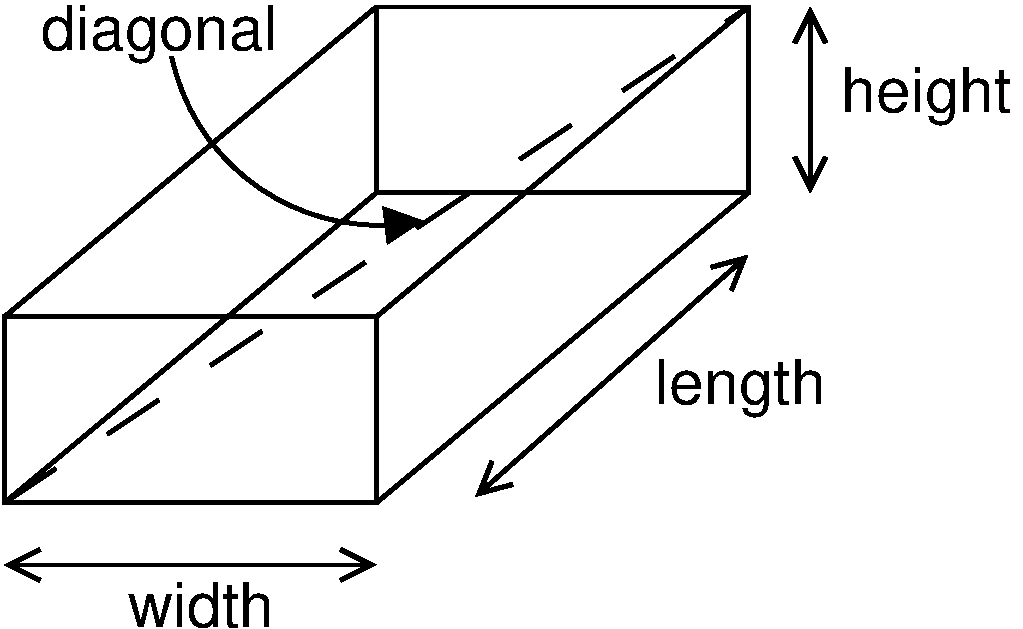
\includegraphics[scale=0.4]{figs/rectangular-prism.pdf}
\caption{Rectangular prism with length, width, height, and diagonal labeled.}
\label{fig.rectangular-prism}
\end{center}
\end{figure}

Write a program with these methods, all of which take the length, width, and height of the box as their three parameters and return a \java{double} result:

\begin{description}
\item \java{getVolume} \hfill \\ Returns the volume of the box.
\item \java{getSurfaceArea} \hfill \\ Returns the surface area of the box.
\item \java{getDiagonal} \hfill \\ Returns the diagonal distance of the box---the distance from the bottom left front corner of the box to the top right back corner.
\end{description}

The \java{main} method will prompt the user to enter the length, width, and height of a box and read them. It will then calculate and print the volume, surface area, and diagonal distance, properly labeled.

Here is an example of what the output might look like. Your program's output does not have to be identical to this, but it must reflect the same information:

\begin{stdout}
Enter length of box: 7
Enter width of box: 3.5
Enter height of box: 4

Volume: 98.00 cubic units
Surface area: 133.00 square units
Diagonal distance: 8.79 units
\end{stdout}

\end{exercise}

\begin{exercise}
The {\em Pythagorean distance} between points $(x_1, y_1)$ and $(x_2, y_2)$ is calculated as $\sqrt {(x_1-x_2)^2 + (y_1-y_2)^2}$. The code to find the Pythagorean distance is in the {\em Think Java 2nd Edition} book. Take the code from the book---or write it yourself---as a method named \java{distance} that takes four parameters (the coordinates of the two points) and returns the Pythagorean distance between those points. All the parameters and the return value are \java{double}.

Another way to measure the distance between two points is the ``city block'' distance: the sum of the absolute $x$ distance plus the absolute $y$ distance:
\begin{equation*}
|x_1 - x_2| + |y_1 - y_2|
\end{equation*}

For example, the city block distance from (1.5, 7) to (5, 2) is 8.5---the $x$ distance is 3.5 ($|1.5 - 5|$) and the $y$ distance is five ($|7 - 2|$).

Write a method named \java{cityBlockDistance} that takes the coordinates of the two points and returns the city block distance between them. All the parameters and the return value are \java{double}. {\em Hint:} Use \java{Math.abs} to calculate absolute value.

The \java{main} method will prompt the user to enter the coordinates; it will then calculate the Pythagorean distance using the \java{distance} method and print the returned result. Finally, \java{main} will call the \java{cityBlockDistance} method to calculate the city block distance and then print the returned result.
\end{exercise}

\begin{exercise}
The Pythagorean and city block distances are fine for a two-dimensional grid, but when you want to find the distance between two points on the spherical earth, you don't use a straight line. Instead, you calculate the {\bf great circle distance} from the latitude and longitude of the points.

Here is the formula where $r$ is the radius of earth in kilometers (6371.009), the first point's latitude and longitude are $lat_1$, $lon_1$ and the second point's latitude and longitude are  $lat_2$, $lon_2$:

\begin{equation*}
d = r\cdot cos^{-1}(sin(lat_1)\cdot sin(lat_2) + cos(lat_1)\cdot cos(lat_2)\cdot cos(lon_1 - lon_2))
\end{equation*}

{\bf Important!} The latitude and longitude in this formula are measured in {\em radians}, not degrees.

Write a method named \java{greatCircleDistance} which takes the latitude and longitude of two points {\em in degrees} as its four parameters and returns the great circle distance, which will be in kilometers.

You will also write a method named \java{kmToMiles} which takes as its single parameter a number of kilometers and returns the equivalent number of miles by multiplying by 0.621371.

Here are the latitude and longitude (in degrees) of several cities:
\begin{itemize}
\item San Jos\'e, California, USA: 37.333, -121.9
\item Los Angeles, California, USA: 34.05, -118.25
\item Seoul, South Korea: 37.56, 126.99
\item Vienna, Austria: 48.2, 16.367
\end{itemize}

Use this information to write the \java{main} method, which will calculate and print, properly labeled, the distance from San Jos\'e to Los Angeles and the distance from Seoul to Vienna. Print the distances in both kilometers and miles.

Here is the expected output:

\begin{stdout}
Distance from San Jose to Los Angeles: 492 km (306 miles)
Distance from Seoul to Vienna: 8277 km (5143 miles)
\end{stdout}

\end{exercise}

